\documentclass[ngerman]{scrbook}
% scrbook lacks \abstract
% Other differences:
% https://tex.stackexchange.com/questions/36988/regarding-the-book-report-and-article-document-classes-what-are-the-mai

\KOMAoptions{
    paper=a4,
    pagesize=auto,
    headsepline=true, % see pagestyle
    numbers=noendperiod,
    %toc=chapterentrywithdots, % prefer tocstyle
    listof=totoc,
    %listof=entryprefix,
    % Kapitel N
    % Überschrift
    %headings=openright,
    headings=big,%twolinechapter,
    chapterprefix=true,
    parskip=full,
    twoside=true,
    fontsize=12pt,
    DIV=15,
    %DIV=calc,
    % Für die PDF-Variante brauche ich keinen BCOR.
    BCOR=10mm,
    %BCOR=8.25mm,
    %BCOR=0mm,
    headinclude=true,
    footinclude=false,
}

%\usepackage{pdfcomment}

\setkomafont{dictumtext}{\itshape\small}
\setkomafont{dictumauthor}{\normalfont}
\renewcommand*\dictumwidth{\linewidth}
\renewcommand*\dictumauthorformat[1]{--- #1}
\renewcommand*\dictumrule{}

\PassOptionsToPackage{ngerman}{babel}
    \usepackage{babel}
\PassOptionsToPackage{T1}{fontenc}
    \usepackage{fontenc}
\PassOptionsToPackage{utf8}{inputenc}
    \usepackage{inputenc}
\PassOptionsToPackage{dvipsnames,pdftex,svgnames,table,usenames}{xcolor}
    \usepackage{xcolor}

\newcommand{\myauthor}{Kai Kühne}  %% also used for PDF metadata (hyperref)
\newcommand{\mycolorlinks}{true}  %% "true" or "false"
%\newcommand{\mydispositioncolor}{30,103,182}
%\newcommand{\mydispositioncolor}{34, 72, 112}
%\newcommand{\mydispositioncolor}{0, 105, 146}
%\newcommand{\mydispositioncolor}{14, 121, 178}
%\newcommand{\mydispositioncolor}{173, 52, 62} % red
%\newcommand{\mydispositioncolor}{12, 116, 137}
%\newcommand{\mydispositioncolor}{35, 100, 170}
%\newcommand{\mydispositioncolor}{0, 52, 89}
%\newcommand{\mydispositioncolor}{24, 48, 89}
%\newcommand{\mydispositioncolor}{39, 111, 191}
\newcommand{\mydispositioncolor}{22, 96, 136}
%\newcommand{\mydispositioncolor}{2, 57, 74}
%\newcommand{\mydispositioncolor}{201, 34, 18}
\newcommand{\secondcolor}{62, 124, 192}
\newcommand{\thirdcolor}{100, 151, 208}
%\newcommand{\mykeywords}{KEYWORDS}  %% also used for PDF metadata (hyperref)
\newcommand{\mysubject}{Master Thesis}  %% also used for PDF metadata (hyperref)
\newcommand{\mytitle}{Entwicklung einer auf Web-Standards basierenden Multiplayer-Online-Plattform für emulierte $($S$)$NES-Konsolenspiele}

\usepackage{xargs}
\usepackage[colorinlistoftodos,prependcaption,textsize=scriptsize]{todonotes}
\newcommandx{\unsure}[2][1=]{\todo[linecolor=red,backgroundcolor=red!25,bordercolor=red,#1]{#2}}
\newcommandx{\change}[2][1=]{\todo[linecolor=blue,backgroundcolor=blue!25,bordercolor=blue,#1]{#2}}
\newcommandx{\info}[2][1=]{\todo[linecolor=OliveGreen,backgroundcolor=OliveGreen!25,bordercolor=OliveGreen,#1]{#2}}
\newcommandx{\improvement}[2][1=]{\todo[linecolor=Plum,backgroundcolor=Plum!25,bordercolor=Plum,#1]{#2}}
\newcommandx{\thiswillnotshow}[2][1=]{\todo[disable,#1]{#2}}

\definecolor{DispositionColor}{RGB}{\mydispositioncolor} %% used for links and so forth in screen-version
\definecolor{DispositionColor2}{RGB}{\secondcolor}
\definecolor{ChapterNumber}{RGB}{192, 214, 223}
%{187, 203, 203}
%\definecolor{textcolor}{cmyk}{0.77, 0.71, 0.66, 0.25}
%\definecolor{textcolor}{RGB}{19, 49, 92}
\definecolor{textcolor}{RGB}{13, 31, 45}
\definecolor{grey}{RGB}{237,235,236}
\definecolor{grey2}{cmyk}{0.17, 0.12, 0.10, 0.00}
\definecolor{madang}{cmyk}{.20, 0, .34, 0}
\definecolor{grey3}{gray}{0.8}
\color{textcolor}
\addtokomafont{disposition}{\color{DispositionColor}}
\addtokomafont{caption}{\color{DispositionColor}\footnotesize}
\addtokomafont{captionlabel}{\color{DispositionColor}}

% https://tex.stackexchange.com/questions/20246/sectioning-bibliography-by-type-of-referred-item
\PassOptionsToPackage{%
    abbreviate=true, % (true, false)
    defernumbers=true, %
    backend=biber,
    backref=true,
    backrefsetstyle=setonly,
    backrefstyle=three, % (none, three, two, two+, three+, all+)
    %dashed=false,
    hyperref=true,
    indexing=false,
    language=auto,
    maxbibnames=10, % default: 3, et al.
    natbib=true,
    punctfont=false, %
    refsection=none, % (part, chapter, section, subsection)
    refsegment=none, % (none, part, chapter, section, subsection)
    sorting=nyt,
    % https://www.sharelatex.com/learn/Biblatex_bibliography_styles
    style=authortitle, %  numeric-comp, % authortitle, numeric-comp
}{biblatex}
    \usepackage{biblatex}
\addbibresource{Masterarbeit.bib}

% FIXME: Add every entry from bib file, just to see them in the pdf.
\nocite{*}

\usepackage[
    bookmarks=false,
    bookmarksopen=false,
    %pagebackref=true,
    pdfpagemode=UseNone, % UseNone, UseOutlines, UseThumbs, FullScreen
    plainpages=false,
    unicode=true,
    % colors: https://secure.wikimedia.org/wikibooks/en/wiki/LaTeX/Colors
    urlcolor=DispositionColor,
    linkcolor=DispositionColor,
    citecolor=DispositionColor,
    anchorcolor=DispositionColor,
    colorlinks=\mycolorlinks,
]{hyperref}

\AtEveryCitekey{%<- This % is needed
\ifciteseen{}{\defcounter{maxnames}{6}\clearfield{namehash}}}

%% all strings need to be loaded after hyperref was loaded with unicode support
%% if not the field is garbled in the output for characters like ČŽĆŠĐ
\hypersetup{
    pdftitle={\mytitle}, %
    pdfauthor={\myauthor}, %
    pdfsubject={\mysubject}, %
    %pdfcreator={Accomplished with: pdfLaTeX, biber, and hyperref-package. No animals, MS-EULA or BSA-rules were harmed.},
    pdfproducer={\myauthor},
}

\setkomafont{section}{\LARGE}
\setkomafont{subsection}{\Large}
\setkomafont{subsubsection}{\large}
\setkomafont{paragraph}{\large}
\setkomafont{subparagraph}{\large}

% http://ctan.math.utah.edu/ctan/tex-archive/macros/latex/contrib/koma-script/doc/tocstyle.pdf
% http://mirror.utexas.edu/ctan/macros/latex/contrib/tocloft/tocloft.pdf
\usepackage{tocstyle}
\usetocstyle{allwithdot}

\usepackage{pgfplots}

\usepackage{mdframed}

% Comment-Column
%\usepackage{scrlayer-notecolumn}
% marginpar
% marginline
% https://tex.stackexchange.com/questions/232629/first-paragraph-indented-after-section-title-in-margin


% https://mirror.hmc.edu/ctan/macros/latex/contrib/tcolorbox/tcolorbox.pdf
\usepackage{tcolorbox}

\usepackage{nameref}

% https://en.wikibooks.org/wiki/LaTeX/Text_Formatting#Hyphenation
% Usage: Super\hyp{}Man
\usepackage{hyphenat}
\usepackage[bottom]{footmisc}
\usepackage{enumitem}
\newcommand\litem[1]{\item{\bfseries #1,\\}}

\setlist{noitemsep}   %% kills the space between items

% Typography
\usepackage[
    activate={true,nocompatibility},
    factor=1100,
    final,
    kerning=true,
    spacing=true,
    tracking=true,
    shrink=10,
    stretch=10,
]{microtype}
\frenchspacing

\usepackage[xindy]{imakeidx}
\makeindex

\usepackage[shortcuts]{extdash}
\renewcommand*\chapterheadstartvskip{\vspace*{.3\textheight}}
\renewcommand*\chapterheadendvskip{\vspace*{.1\textheight}}
\renewcommand*{\chapterformat}{%
  \parbox{\textwidth}{\hfill\chapappifchapterprefix{\ }\thechapter\autodot\enskip}}
\addtokomafont{disposition}{\normalfont\bfseries}
\addtokomafont{chapterprefix}{\fontsize{120}{20}\color{ChapterNumber}\mdseries\scshape}

% Head & Foot
%\usepackage[automark]{scrlayer-scrpage}
%\ihead{Peter Musterheinzel}
%\ohead{Seitenstile mit \KOMAScript}
%\ifoot*{Verlag Naseblau, Irgendwo}
%\pagestyle{scrheadings}
%\setkomafont{pageheadfoot}{\small}
%\setkomafont{pagehead}{\bfseries}
%\pagestyle{scrheadings}
\pagestyle{headings}

% Chapters
\AtBeginDocument{\renewcommand{\partname}{}} % "Kapitel 1" -> "1"
\renewcommand{\partformat}{}
\addtokomafont{part}{\fontsize{65}{55}\selectfont}
\AtBeginDocument{\renewcommand{\chaptername}{}} % "Kapitel 1" -> "1"
\renewcommand*{\raggedchapter}{\raggedleft} % Align right
\addtokomafont{chapter}{\fontsize{45}{35}\selectfont}

\usepackage{textcomp} % fix warning with missing font shapes
\usepackage{scrhack} % fix warnings when using KOMA with listings package
\usepackage{xspace} % to get the spacing after macros right
\usepackage{mparhack} % get marginpar right
\usepackage[latest]{latexrelease} % will be used once available in more distributions (ISSUE #107)

% https://github.com/novoid/LaTeX-KOMA-template
\usepackage{eso-pic}
% \unit[42]{m}
% \unitfrac[100]{km}{h}
\usepackage{units}

\usepackage[rightcaption]{sidecap}
\newcommand{\myfig}[5]{
%% example:
% \myfig{}%% filename in figures folder
%       {width=0.5\textwidth,height=0.5\textheight}%% maximum width/height, aspect ratio will be kept
%       {}%% caption
%       {}%% optional (short) caption for list of figures
%       {}%% label
\begin{figure}[htb]
  \centering
  \includegraphics[keepaspectratio,#2]{#1}
  \caption[#4]{#3}
  \label{#5} %% NOTE: always label *after* caption!
\end{figure}
}

\usepackage[rightcaption]{sidecap}
\newcommand{\myfigcool}[5]{
%% example:
% \myfig{}%% filename in figures folder
\begin{SCfigure}[0.5][htb]
  \caption[#4]{#3}
  \includegraphics[keepaspectratio,#2]{#1}
\end{SCfigure}
}

\usepackage{tabularx} % better tables
    \setlength{\extrarowheight}{3pt} % increase table row height
\newcommand{\tableheadline}[1]{\multicolumn{1}{c}{\spacedlowsmallcaps{#1}}}
\newcommand{\myfloatalign}{\centering} % to be used with each float for alignment
\usepackage{caption}
\captionsetup{font=small}
\usepackage{subfig}

% Text: Align left
%\usepackage[document]{ragged2e}

\pdfcompresslevel=9
\pdfadjustspacing=1

\PassOptionsToPackage{pdftex}{graphicx}
    \usepackage{graphicx}
    \graphicspath{{Abbildungen/}}

% Serif
\usepackage[sc]{mathpazo} % Palatino with small caps [sc] and old style figures [osf]

%\overfullrule=2cm

% Sans-Serif
%\usepackage[sfdefault]{FiraSans}
\usepackage{FiraSans}

\usepackage{setspace}
%\singlespacing
\onehalfspacing
%\doublespacing
%\setstretch{1.1}

\usepackage{blindtext}

\usepackage[babel=true,strict=true,english=american,german=guillemets]{csquotes}
%\usepackage[titletoc,toc,page]{appendix}
%\renewcommand{\appendixtocname}{Anhang}
%\renewcommand{\appendixpagename}{Anhang}
\usepackage{pdflscape}
\usepackage{pdfpages}

\newcounter{dummy} % necessary for correct hyperlinks (to index, bib, etc.)
\newlength{\abcd} % for ab..z string length calculation

% http://mirrors.ibiblio.org/CTAN/macros/latex/contrib/glossaries/glossariesbegin.pdf
% http://mirrors.ibiblio.org/CTAN/macros/latex/contrib/glossaries/glossaries-user.pdf

\usepackage[
    acronym,
    %nomain,
    nonumberlist,
    nopostdot,
    shortcuts,
    smallcaps,
    toc,
    xindy,
]{glossaries}

\makeglossaries

% Usage: \gls{foo} -> Will automatically place long version first once, then short.
% Uses Small caps.
\setacronymstyle{long-sc-short}
\setglossarystyle{list}

\newacronym{http}{Http}{Hyper Text Transfer Protocol, \href{https://tools.ietf.org/html/rfc2616}{RFC 2616}}
\newacronym{mpeg-1}{Mpeg-1}{\todo{}Moving Picture Experts Group Phase 1}
\newacronym{nat}{Nat}{Network Address Translation, \href{https://tools.ietf.org/html/rfc1631}{RFC 1631}}
\newacronym{www}{Www}{World Wide Web}
\newacronym{nes}{Nes}{Nintendo Entertainment System}
\newacronym{snes}{Snes}{Super Nintendo Entertainment System}
\newacronym{stun}{Stun}{Session Traversal Utilities for \gls{nat}, \href{https://tools.ietf.org/html/rfc5389}{RFC 5389}}
\newacronym{turn}{Turn}{Traversal Using Relays around \gls{nat}, \href{https://tools.ietf.org/html/rfc5766}{RFC 5766}}
\newacronym{rom}{Rom}{Read-Only Memory}
\newacronym{gui}{Gui}{Graphical User Interface}
\newacronym{webrtc}{WebRTC}{Web Real-Time Communications}
\newacronym{ice}{Ice}{Interactive Connectivity Establishment}
\newacronym{crud}{Crud}{Menge der häufigsten Operationen einer (Web-)API: Create, Read, Update, Delete}
\newacronym{json}{Json}{JavaScript Object Notation. Weitverbreitetes Format zur (De)Serialisierung von Nachrichten}

\newglossaryentry{accessibility}{name={Accessibility},description={\todo{}}}
\newglossaryentry{canvas}{name={Canvas},description={\todo{}}}
\newglossaryentry{websockets}{name={WebSockets},description={\todo{}, \href{https://tools.ietf.org/html/rfc6455}{RFC 6455}}}
\newglossaryentry{controller}{name={Controller},description={Gerät zur Steuerung von Computerspielen. Bei alten Konsolen über Kabel verbunden}}
\newglossaryentry{django}{name={Django},description={Web-Framework für die Programmiersprache Python}}
\newglossaryentry{docker}{name={Docker},description={Plattform zur Erstellung und Verwaltung von Software-Containern}}
\newglossaryentry{emulator}{name={Emulator},description={Computer-Programm zur Emulation von Konsolenspielen}}
\newglossaryentry{host}{name={Host},description={Dienstanbietender Teilnehmer in einem Computer-Netzwerk}}
\newglossaryentry{LLVM}{name={Llvm},description={Compiler-System basierend auf den Konzepten virtueller Maschinen. Beinhaltet Compiler (clang) und arbeitet mit einer Zwischensprache, die es erlaubt, während des Linkvorgangs Optimierungen durchzuführen.}}


\usepackage{listings}
\usepackage{soul}
\usepackage{url}
\usepackage[all]{hypcap}


\setcounter{tocdepth}{1}
\setcounter{secnumdepth}{4}

\lstset{
language=Python,                  % choose the language of the code
basicstyle=\footnotesize,       % the size of the fonts that are used for the code
numbers=left,                  % where to put the line-numbers
%numberstyle=\footnotesize,      % the size of the fonts that are used for the line-numbers
stepnumber=2,                   % the step between two line-numbers. If it's 1 each line will be numbered
numbersep=5pt,                  % how far the line-numbers are from the code
backgroundcolor=\color{grey},   % choose the background color. You must add \usepackage{color}
showspaces=false,               % show spaces adding particular underscores
showstringspaces=false,         % underline spaces within strings
showtabs=false,                 % show tabs within strings adding particular underscores
%frame=single,                  % adds a frame around the code
tabsize=4,                      % sets default tabsize to 2 spaces
captionpos=b,                   % sets the caption-position to bottom
breaklines=true,                % sets automatic line breaking
breakatwhitespace=false,        % sets if automatic breaks should only happen at whitespace
title=\lstname,                 % show the filename of files included with \lstinputlisting; also try caption instead of title
escapeinside={\%*}{*)},         % if you want to add a comment within your code
%%morekeywords={*,...}          % if you want to add more keywords to the set
literate=%
    {€}{\euro}1%
    {§}{\S}1%
    %{°}{\textdegree{}}1%
    {ä}{{\"a}}1%
    {ö}{{\"o}}1%
    {ü}{{\"u}}1%
    {ß}{{\ss}}1%
    {Ä}{{\"A}}1%
    {Ö}{{\"O}}1%
    {Ü}{{\"U}}1%
    %{µ}{\textmu}1%
    %{¹}{{\textsuperscript{1}}}1%
    %{²}{{\textsuperscript{2}}}1%
    %{³}{{\textsuperscript{3}}}1%
    %{¼}{\textonequarter}1%
    %{½}{\textonehalf}1%
    %{¢}{\textcent}1%
}

\renewcommand*\listfigurename{List of figures}

\newcommand{\HRule}{\rule{\linewidth}{0.5mm}}

% Bullets all the way down...
\renewcommand{\labelitemi}{$\bullet$}
\renewcommand{\labelitemii}{$\bullet$}
\renewcommand{\labelitemiii}{$\bullet$}
\renewcommand{\labelitemiv}{$\bullet$}

\providecommand{\tightlist}{%
  \setlength{\itemsep}{0pt}\setlength{\parskip}{0pt}}

\begin{document}
\frontmatter

\listoftodos[TODO]

%\begin{abstract}
% \end{abstract}

\dedication{%
              Meinem Schnuckelchen\\
              in ewiger Liebe\\
              von Deinem Hasenboppelchen.}

\begin{titlepage}
\vspace*{\fill}
\begin{center}
\LARGE
Masterarbeit\\
\Large
\textbf{\mytitle}\\[1cm]
\large
\myauthor{}\\
798797\\[1cm]
Beuth Hochschule für Technik Berlin\\
Fachbereich VI -- Informatik und Medien
\vfill
\vfill
Berlin, \today
\normalsize
\vfill
\vfill
\begin{tabular}{rl}
Betreuung: & Herr Dipl.-Inform. Hans-Georg Reimer (LB)\\
Begutachtung: & Herr Prof. Dr. Hildebrand
\end{tabular}
\end{center}
\vspace*{\fill}
\end{titlepage}

\tableofcontents
\cleardoublepage

\mainmatter

\setchapterpreamble[uc][.75\textwidth]{%
\dictum[Lewis Carroll, \textit{Alice in Wonderland}]{%
``Begin at the beginning,'' the King said, gravely, ``and go on till you come to an end; then stop.''}\vskip1em}

\chapter{Einleitung}\label{einleitung}

Nach der Krise der Videospiel-Industrie Mitte der achtziger Jahre hatte
Nintendo mit der Veröffentlichung des \gls{nes} eine Konsole für
Videospiele auf den Markt gebracht, die sich millionenfach verkaufte.
Dabei führte das Unternehmen weltbekannte Marken wie Mario,
\index{Donkey Kong} und Zelda ein, mit denen das Unternehmen bis zum
heutigen Tag erfolgreich ist. In den 90er Jahren wurde der Nachfolger
auf den Markt gebracht, das \gls{snes}. Beide Systeme verkauften sich
zusammen weltweit über 100 Millionen mal und sind damit die
erfolgreichsten Systeme ihrer Generation. Insgesamt wurden für beide
Systeme ca. 1495 Spiele entwickelt und lizensiert; darunter
Singleplayer-Klassiker wie Super Metroid oder \enquote{Mega Man}.
Gespielt werden konnte aber nicht nur allein: Die Konsolen wurden von
vornherein für mehrere Spieler ausgelegt und verfügen über zwei
Anschlüsse für Controller. Dies führte dazu, dass viele Spiele sowohl
einen Singleplayer- als auch einen Multiplayer-Modus beinhalteten, der
es ermöglichte, mit mehreren Spielern an der Konsole zu spielen.

Mittlerweile existieren mindestens zwei weitere erfolgreiche
Videospiel-Konsolen: Die Xbox One von Microsoft und die PlayStation 4
von Sony. Wie auch schon das \gls{nes} unterstützen beide Systeme
mehrere Spieler, über entsprechende Controller, die mit der Konsole
gekoppelt werden. Die technologische Entwicklung seit den 80er und 90er
Jahren ist gut am Internet abzulesen: Damals galt ein 28.8k-Modem als
Highspeed-Gerät. Heutzutage sind breitbandige Internetanschlüsse
großflächig verfügbar. Dieser technologische Fortschritt ermöglicht es,
größere Datenmengen übers Internet zu übertragen -- z. B. Daten eines
Multiplayer-Spiels. Man spielt nicht mehr exklusiv im eigenen Wohnzimmer
oder auf einer LAN-Party gemeinsam miteinander, sondern kann dies über
das Internet und über Landesgrenzen hinweg tun. Dazu haben Microsoft und
Sony jeweils kostenpflichtige Online-Plattformen geschaffen, über die
Spieler miteinander über verschiedenste Kanäle interagieren -- und, viel
wichtiger -- miteinander spielen können. Die Plattformen bieten einen
Treffpunkt der Kommunikation und Vermittlung und stellen für die
Spiele-Entwickler Dienste wie Spiel-Lobbys und Matchmaking bereit.

Eine bemerkenswerte Eigenschaft beider Plattformen ist deren einfache
Handhabung: Sie machen es den Spielern sehr einfach, gemeinsam über das
Internet miteinander zu spielen. Die Plattformnutzer müssen über keine
speziellen Kenntnisse verfügen, müssen keine zusätzliche Software
installieren oder etwa darin geübt sein, einen dedizierten Game-Server
aufsetzen. Mitglieder der Plattform können sich auf das Spielen
konzentrieren. Aktuelle Spiele-Titel können ohne große Hürden über die
beschriebenen Plattformen gespielt werden. Eine Plattform für
\gls{snes}-Spiele, die einen vergleichbaren Komfort bietet, existiert
bislang nicht.

\section{Motivation}\label{motivation}

Möchte man am PC ein Konsolenspiel, z. B. Super Mario, spielen, benötigt
man neben dem eigentlichen Spiel auch ein Programm, mit dem das Spiel
ausgeführt werden kann: einen Emulator. Einen geeigneten Emulator
auszuwählen ist nicht einfach: Allein für das \gls{snes} existieren mehr
als ein Dutzend Emulatoren für verschiedenste Betriebssysteme (vgl.
\cite{snes-emulator-list}), die sich in der Genauigkeit der Emulation,
der Kompatibilität und weiteren Aspekten unterschieden und von denen
partiell zusätzliche Ableger (Forks) existieren (FIXME). Ein Teil der
Emulatoren verfügt über einen Multiplayer-Modus. Mit dem Problem, dass
die verschiedenen Emulatoren untereinander meist inkompatibel sind
(FIXME). Auch bei komplexeren Emulationssystemen wie RetroArch, das
viele Emulatoren enthält und um eine eigens geschaffene Netplay-Funktion
erweitert, ist die Kompatibilität nicht garantiert (vgl.
\cite{retroarch-netplay-comp}). Um erfolgreich ein \gls{snes}-Spiel im
Multiplayer-Modus gespielt werden, müssen alle Spieler im Idealfall den
gleichen Emulator in der selben Version verwenden. Sofern die
verwendeten Emulatoren unteinander kompatibel sind, existieren weitere
Hürden, die für einen Anwender ohne technischen Hintergrund nicht ohne
Weiteres zu lösen sind. Ein möglicher Ablauf zum Erstellen eines Spiels:

\begin{itemize}
\tightlist
\item
  Einer der Spieler wird als \gls{host} bestimmt und startet den
  Emulator im Netzwerk-Modus.
\item
  Der Host muss dabei sicherstellen, dass der spezifische Port, auf dem
  der Prozess läuft, von allen Mitspielern über das Netzwerk erreichbar
  ist. Falls der Host-Ssieler sich in einem Netzwerk befindet, dessen
  Routing auf \gls{nat} basiert, muss eine Port-Weiterleitung für den
  Emulator-Prozess eingerichtet werden, der auf dem PC des Host-Spielers
  läuft. Dazu muss die verwendete Portnummer des Emulators bekannt und
  eine Port-Weiterleitung im Administrationsbereich des Routers
  konfiguriert sein. Für das beschriebene Szenario ist die korrekte
  \gls{nat}-Konfiguration Voraussetzung für das Spielen im
  Multiplayer-Modus.
\item
  Wenn der ausgewählte Emulator über keine Funktion verfügt, um
  Netzwerkspiele aufzulisten, benötigen alle Mitspieler die IP-Adresse
  des Host-Spielers, um eine Verbindung herzustellen.
\item
  Der Host-Spieler muss die eigene öffentliche IP-Adresse ermitteln und
  seinen Mitspielern mitteilen.
\item
  Die Mitspieler verbinden sich mit dem Host-Spieler über die Eingabe
  der IP-Adresse des Hosts im entsprechenden Dialog der
  Benutzeroberfläche des verwendeten Emulators.
\end{itemize}

\section{Zielsetzung}\label{zielsetzung}

Im Zuge der immer größer werdenden Verfügbarkeit von breitbandigen
Internetanschlüssen entstehen neue Chancen für die Entwicklung
interessanter neuer Lösungen. Mit den Chancen stellen sich aber auch
neue Herausforderungen, für deren Lösung neue Technologien geschaffen
werden. Ein Teilbereich ist das \gls{www}, das eine kontinuierliche
Weiterentwicklung erfährt und sich die Computer-Nutzung immer mehr in
den Internet-Browser verlagert.

Ablesen lässt sich die Weiterentwicklung der Web-Technologien zum
Beispiel durch die Entwicklung neuer Standards- und Protokolle. Der
Internet-Browser hat nahezu den Funktionsumfang eins Desktop-Systems und
kann ein breites Spektrum von Anwendungsfällen abdecken. Das Abspielen
von Audio- und Videodaten, die direkte Kommunikation zwischen Browsern
und das Ausführen von komplexen 3D-Anwendungen ist mittlerweile möglich.

Diese Arbeit untersucht die Frage, ob die aktuell verfügbaren
Web-Standards die Anforderungen für die Entwicklung einer
Multiplayer-Plattform für \gls{snes}-Spiele erfüllen und welche
Technologien wie kombiniert werden müssen, um ein funktionales System zu
schaffen. Die zentralen Aspekte sind die Auswahl, die Kombination und
die Integration der verschiedenen Technologien zu einem Gesamtsystem
bestehend aus verschiedenen Komponenten, die alle im Zuge dieser Arbeit
entwickelt werden.

Der Fokus liegt dabei auf der Entwicklung einer funktionalen
Web-Plattform mit den wichtigsten Basisfunktionen, die aufgrund einer
sauberen Architektur leicht um neue Funktionen zu erweitern ist.

\section{Vorgehensweise}\label{vorgehensweise}

\begin{enumerate}
\def\labelenumi{\arabic{enumi}.}
\tightlist
\item
  \textbf{Grundlagen} Einarbeitung und Erläuterung der technischen
  Grundlagen, die für die Lösung der Zielsetzung notwendig sein können.
  Dies umfasst verschiedene Web-Technologien auf der einen Seite und
  Emulationssysteme auf der anderen Seite.
\item
  \textbf{Zieldefinition} Genaue Festlegung des Funktionsumfangs des zu
  erstellenden Systems.
\item
  \textbf{Herausforderungen} Ableitung der zu lösenden Teilprobleme, die
  sich aus den definierten Zielen ergeben.
\item
  \textbf{Lösungsansätze} Untersuchen, ob und welche Teillösungen für
  die im vorherigen Abschnitt beschriebenen Probleme existieren.
  Vorstellen von Lösungsansätzen, die ggf. auf vorhandenen Teillösungen
  aufbauen oder diese erweitern. Gewählten Lösungsansatz vorstellen und
  mögliche Alternativen aufzeigen.
\item
  \textbf{Methodik} Beschreibung der Umsetzung.
\item
  \textbf{Konzeption} Entwurf der Benutzeroberfläche, Definition der
  System-Komponenten und der Software-Architektur.
\item
  \textbf{Implementierung} Technische Beschreibung der entwickelten
  Lösung mit Fokus auf ausgewählte Aspekte der Implementierung.
\item
  \textbf{Evaluation} Überprüfung und Bewertung der Lösung im Hinblick
  auf das Erreichen der definierten Ziele.
\item
  \textbf{Fazit} Zusammenfassung und Bewertung der Arbeit sowie
  Vorstellen von Erweiterungsmöglichkeiten.
\end{enumerate}

\chapter{Grundlagen}\label{grundlagen}

Inhalt dieses Kapitels ist eine Einführung in die technischen Grundlagen
dieser Arbeit. Es werden die wichtigsten Aspekte und Technologien
erläutert und für das Lösungsumfeld essentielle Begriffe erklärt. Die
Erläuterungen schaffen ein Grundverständnis für die in den nachfolgenden
Kapiteln behandelten Aspekte und sind für eine Beurteilung der
entwickelten Lösung notwendig. Schwerpunkte sind für die Zielsetzung
potentiell geeignete Web-Technologien, Emulatoren \& ROMs und
Grundbegriffe aus dem Bereich der Kommunikation in Computer-Netzwerken.

\section{SNES-Emulation}\label{snes-emulation}

Wie eingangs erwähnt, sind zum Spielen von \gls{snes}-Spielen am
Computer zwei Dinge notwendig: Ein Emulationsprogramm --- auch
\gls{emulator} genannt --- und das jeweilige Konsolenspiel, das
ausgeführt werden soll.

Der Emulator ist ein Software-Programm, das die Ausführung von Spielen
ermöglicht, die ursprünglich für eine spezifische Konsole entwickelt und
auf diese hin optimiert worden sind. Bei der Emulation wird die Hardware
der jeweiligen Konsole nachgeahmt. Die verschiedenen physischen
Komponenten der Konsole (CPU, Soundchip, etc.) sind dabei so in Software
implementiert, dass sie sich möglichst so verhalten, wie die
nachzuahmende Hardware. Erst eine exakte Emulation der ursprünglichen
Laufzeitumgebung ermöglicht die Ausführung von unveränderten Spielen in
Form von ROM-Dateien. Durch die Emulation der originalen Hardware kann
ein Großteil der Spiele unverändert ausgeführt werden.

Das Spiel liegt dabei in Form einer Datei vor.
Sie beinhaltet die exakt gleichen Daten, die sich für gewöhnlich auf den
Modulen befinden, die zum Spielen in die Konsolen gesteckt werden
müssen. Zum Kopieren der Daten existiert spezielle Hardware, mit denen
eine solche Datei erzeugt werden kann. Dabei wird ein genaues Abbild des
Spielmoduls erzeugt, inklusive der Sektoren und der jeweiligen
Dateisystem-Struktur. Die Dateien werden oft als ROMs bezeichnet, da die
Daten des Spiels innerhalb des Moduls in einem ROM-Chip gespeichert
sind. ROM-Dateien beinhalten neben dem unveränderten Abbild weitere
Metadaten, die ebenfalls in der Datei abgelegt werden. Die genaue
Dateistruktur hängt vom jeweiligen Format der ROM-Datei ab, von denen
eine Vielzahl für verschiedenste Zielsysteme existieren. Am geläufigsten
für das \gls{snes} sind die Dateiformate \emph{SMC} und \emph{SMC}. Um
ein Spiel auszuführen zu können, muss eine ROM-Datei in einen Emulator
geladen werden, der das jeweilige Format unterstützt.

\subsection{Portabilität}\label{portabilituxe4t}

Die bekanntesten und am meisten verwendeten (FIXME: Quelle)
SMES-Emulatoren sind snes9x, zsnes und bsnes. Eine Übersicht über deren
Eigenschaften ist in Tabelle FIXME aufgeführt.

Bemerkenswert ist die Tatsache, dass die Ausführung eines Emulators mit
hoher Genauigkeit (bsnes) sehr rechenintensiv ist.

\begin{longtable}[]{@{}llll@{}}
\toprule
Emulator & Betriebssystem & Genauigkeit &
System-Anforderungen\tabularnewline
\midrule
\endhead
bsnes & Windows, Linux, macOS & Sehr hoch & Hoch\tabularnewline
snes9x & Multi-Plattform & Hoch & Gering\tabularnewline
zsnes & Multi-Plattform & Gering & ~Gering\tabularnewline
RetroArch \\ (snes9x,\\ bsnes) & Multi-Plattform & - &
-\tabularnewline
\bottomrule
\end{longtable}

Quelle:
\url{http://emulation-general.wikia.com/wiki/Super_Nintendo_emulators}

Neben den in der Tabelle aufgeführten Emulatoren existieren jeweils eine
handvoll Varianten (Forks), die verschiedene Verbesserungen oder
Veränderungen hinzufügen oder auch entfernen. Als Beispiel sei hier
\emph{snes9x2000} genannt, eine Re-Implementierung von snes9x in C
(statt C++).

Zusätzlich zu den in der Tabelle aufgeführten Betriebssysteme existieren
Emulatoren auch in Form nativer Apps für das Smartphone, die über die
jeweiligen App Stores bezogen werden können.

Emulatoren können nicht nur auf dem Desktop und dem dem Smartphone
genutzt werden --- mittlerweile ist auch die direkte Ausführung im
Web-Browser möglich. Diese direkte Ausführung basiert auf JavaScript und
weiteren Web-Standards und benötigt darum keine Browser-Plugins. Um
Software im Browser ausführen zu können, muss diese entweder direkt in
JavaScript implementiert sein oder in einer anderen vom Browser
ausführbaren Form vorliegen (FIXME: asm.js oder WebAssembly). Bei den
Projekten RetroArch und xnes findet die zweitgenannte Methode Anwendung:
Der eigentliche Quellcode ist kein JavaScript-Code und muss daher mit
Hilfe eines Übersetzungsprogramms in eine im Browser ausführbare Form
überführt werden. Beide Projekte verwenden für die Übersetzung das
Framework \emph{Emscripten}.

\section{Emscripten}\label{emscripten}

Emscripten ist ein Projekt und ein gleichnamiger Compiler, der es
erlaubt ein Programm, das in Form von LLVM-Bitcode vorliegt,
in JavaScript-Code zu übersetzen. Der JavaScript-Code ist dann
ohne weiteres in einem Web-Browser ausführbar. Bei LLVM-Bitcode handelt
es sich um einen \emph{Zwischencode}, der während des Kompiliervorgangs
mit einem LLVM-Compiler (z. B. \emph{clang}) erzeugt wird. clang kann
verwendet werden, um C/C++-Quellcode zu übersetzen. Grundsätzlich
unterstützt Emscripten aber auch weitere Systeme, sofern diese
LLVM-Bitcode erzeugen. Neben dem JavaScript-Code enthält die erzeugte
Datei auch die Emscripten-Runtime, die für die Ausführung im Browser
benötigt wird.

\myfig{Grundlagen/Emscripten_Funktionsweise}
   {width=0.9\textwidth}
   {Emscripten: Übersetzung eines Programms nach JavaScript.}
   {Emscripten: Funktionsweise}
   {fig:basics_emscripten_moo}

Bei der Übersetzung eines Programms durch Emscripten entsteht ein neues
Programm, das in die eigene Web-Applikation integriert und aufgerufen
werden kann. Der Code läuft dabei direkt im Browser, da das
Original-Programm in ein Format überführt wurde, das direkt im Browser
ausführbar ist. Aktuell unterstütze Formate sind \emph{asm.js} und
\emph{WebAssembly}.

\subsection{Voraussetzungen}\label{voraussetzungen}

Um ein Programm mit Emscripten zu übersetzen und das Ergebnis im Browser
auszuführen, muss das Programm bestimmte Voraussetzungen erfüllen. Denn
selbstverständlich stehen im Browser nicht alle
Programmierschnittstellen zur Verfügung, die auf einem Desktop-System
(z. B. Windows) vorhanden sind. Es handelt sich um eine neue
Laufzeitumgebung, in der viele Funktionen nicht verfügbar sind. Die in
jedem mit Emscripten übersetzenden Programm enthaltene Laufzeitumgebung
implementiert verschiedene Schnittstellen:
Hervorzuheben ist SDL. SDL ist ein Multimedia-Framework, das dank
Emscripten auch im Browser verfügbar ist. Eingesetzt werden kann es für
grafische Darstellungen, Eingabe-Verarbeitung, die Audio-Ausgabe und
weitere. Wenn das Programm über die entsprechenden Funktionen verfügen
soll, müssen diese mit SDL umgesetzt werden. Der Anpassungsaufwand ist,
neben weiteren Aspekten, primär davon abhängig wie hoch der Aufwand der
Portierung des Programms nach SDL ist. Wenn das Projekt groß ist und beispielsweise
OpenGL verwendet wurde, ist der Aufwand sehr hoch. Verwendet das Projekt
bereits SDL, sind gegebenenfalls nur wenige Anpassungen notwendig.

\subsection{Anwendungsbeispiel}\label{anwendungsbeispiel}

Dieser Abschnitt soll das Verständnis von Emscripten und dessen
Funktionsweise durch ein praktisches Beispiel verdeutlichen.

Ein fertiges Tetris-Spiel soll als Webseite online spielbar sein.
Das Projekt soll für die weitere Entwicklung vorbereitet werden.
Bestehen tut das Projekt aus einer HTML-Datei und einer JavaScript-Datei, die
über das HTML-``script''-Element in die HTML-Datei eingebunden wird. Das
Spiel ist in SDL implementiert und verwendet für die grafische
Darstellung, die Audio-Ausgabe und die Eingabe-Verarbeitung die
entsprechenden SDL-Funktionen -- eine Portierung ist nicht notwendig.
Die genannten Programmteile liegen als C-Modul vor und befinden sich
in der Datei \emph{Tetris.c}. Die Struktur des Projekts ist in Abbildung
\ref{fig:basics_emscripten_usage_1} dargestellt.

\myfig{Grundlagen/Emscripten_Verwendung_1}
   {width=0.4\textwidth}
   {Anwendungsbeispiel von Emscripten (1/3)}
   {Emscripten: Verwendung (1/3)}
   {fig:basics_emscripten_usage_1}

Um nun von der JavaScript-Applikation (\emph{App.js}) auf den
eigentlichen Spielcode zuzugreifen, muss dieser mit Emscripten nach
JavaScript übersetzt werden (Abbildung \ref{fig:basics_emscripten_usage_2}).

\myfig{Grundlagen/Emscripten_Verwendung_2}
   {width=0.9\textwidth}
   {Anwendungsbeispiel von Emscripten (2/3)}
   {Emscripten: Verwendung (2/3)}
   {fig:basics_emscripten_usage_2}

Die dabei entstandenen Dateien werden in die HTML-Datei eingebettet. Nun
können die C-Funktionen des Tetris-Moduls direkt aus der JavaScript-App
heraus aufgerufen werden (Abbildung \ref{fig:basics_emscripten_usage_3}).

\myfig{Grundlagen/Emscripten_Verwendung_3}
   {width=0.9\textwidth}
   {Anwendungsbeispiel von Emscripten (3/3)}
   {Emscripten: Verwendung (3/3)}
   {fig:basics_emscripten_usage_3}

\section{Latenz}\label{latenz}

Die Definition des Latenz-Begriffs hängt stark vom Kontext ab, in dem er
gebraucht wird. Für den Benutzer dieser Web-Applikation ist die Latenz
die Zeit, die vergeht, bis eine auf der Oberfläche getätigte Aktion (zum
Beispiel eine Eingabe über die Tastatur) zu einem beobachteten Effekt
auf der Webseite führt. Diese gefühlte ``Gesamtlatenz'' ist von vielen
Faktoren abhängig, von denen viele nicht beinflussbar sind, weil ihnen
physikalische Grenzen gesetzt sind und schon die verwendeten Technologien
Latenzen erzeugen. Beim Versenden von Paketen über das
Netzwerk begrenzt spätestens die Lichtgeschwindigkeit die maximale
Übertragungsgeschwindigkeit: Ein Netzwerkpaket, das über eine
Glasfaserverbindung transportiert wird, legt die Strecke von knapp 6000
km zwischen New York und London in 28 ms zurück, die Paketumlaufzeit
beträgt entsprechend (Round-trip Time, RTT) von 56 ms. Die
Netzwerk-Latenz sollte also nicht unterschätzt werden. Trotzdem ist sie
nur ein Faktor von vielen, den es zu bedenken gilt: Ein Computer-System
besteht aus vielen Komponenten, die untereinander kommunizieren und
Informationen austauschen: Dabei führt jede Berechnung, die eine CPU
zusätzlich ausführen muss, letztlich zu einer höheren Gesamtlatenz.

\myfig{Grundlagen/Latenz}
   {width=0.6\textwidth}
   {Jede der dargestellten Ebenen trägt zu der Gesamtlatenz Applikation bei.}
   {Latenz}
   {fig:basics_latency}

Abbildung \ref{fig:basics_latency} zeigt eine abstrakte Darstellung der Ebenen des Systems
und den Übergängen zwischen den Ebenen, an denen eine spürbare Latenz
vorhanden sein wird. Wichtig ist die Tatsache, dass das Auftreten von
Latenzen grundsätzlich unvermeidlich und teilweise nicht beeinflussbar
ist. Deswegen sollten diejenigen Stellen analysiert werden, auf die
Einfluss genommen werden kann. Dabei sollte abgewogen werden, ob sich
der durch die Optimierung enstandende Mehraufwand lohnt und dies bei der
Systemplanung berücksichtigen.

\section{Single-Page Applications}\label{single-page-applications}

Single-Page Applikations, kurz SPAs, sind Web-Applikationen, die aus
einer HTML-Seite bestehen, die vom Webserver an den Client ausgeliefert
wird. Alle nachfolgenden benötigten Ressourcen werden von der
Applikation asynchron nachgeladen und der Inhalt der HTML-Seite
\emph{in-place} verändert. Das Frontend wird dabei meist in JavaScript
und unter Zuhilfenahme von entsprechenden Frontend-Frameworks, wie z. B.
React.js oder Vue.js, implementiert. Das Backend-System bietet in einer
SPA meist eine REST-API an: Die Essenz davon ist die Bereitstellung und
der Zugriff auf die Datenbasis der Applikation über HTTP. Dabei werden
den verschiedenen HTTP-Methoden (GET, POST, etc.) den entsprechenden
\acrshort{crud}-Operationen zugeordnet. Eine REST-API wird als vom Frontend
unabhängiger Netzwerkdienst betrieben, auf den das Frontend mit
verschiedenen Methoden zugreift, um Datensätze über die definierte
REST-Schnittstelle abzufragen oder Änderungen in der Datenbank zu
persistieren. Die Kommunikation zwischen Frontend und Backend in einer
SPA erfolgt meist über AJAX bzw. über den in JavaScript eingebauten
XmlHttpRequest-Mechanismus. Als Transportprotokoll für REST-Dienste
würde ursprünglich XML verwendet; inzwischen setzt sich \acrshort{json}
immer mehr durch.

\todo[inline]{Setze ich zu viel voraus?
              Unterschied zu traditioneller Architektur mehr hervorheben?
              Evtl. noch ein Diagramm? Ich wollte den Part nicht so lang machen,
              da WebRTC sehr detailliert erklärt wird / werden muss.}

\section{Das Realtime-Web}\label{das-realtime-web}

Eine Echtzeit-Web-Applikation setzt auf den Prinzipien einer SPA auf.
Der Unterschied: SPAs basieren darauf, dass Anfragen stets vom Frontend
ans Backend gesendet und von diesem beantwortet werden. Eine
Datenübertragung, die vom Backend initiiert wird, existiert bei dieser
Architektur nicht: Das Frontend muss regelmäßig beim Backend anfragen,
ob aktualisierte Daten vorliegen (Polling).

Bei Realtime-Web-Apps erfolgt die Kommunikation in beide Richtungen. Das
bedeutet, dass Änderungen vom Backend direkt im Frontend ersichtlich
werden, da ein Kommunikationskanal verwendet wird, bei dem der Server
dem Client Nachrichten senden kann. Daten müssen nicht regelmäßig vom
Frontend angefragt werden, sondern werden vom Backend an das Frontend
gesendet, sobald diese verfügbar sind (Push).

Für die Kommunikation zwischen Server und Client bietet sich z. B. der
Einsatz von WebSockets an, da es ein effizienter Transport-Mechanismus
mit geringer Latenz ist und Multiplexing beherrscht.

\subsection{Server-Sent Events (SSE)}\label{server-sent-events-sse}

Server-Sent Events ermöglichen das Streamen von textbasierten Daten vom
Server zum Client (Browser). Die Datenübertragung erfolgt über eine
Verbindung, die einmal aufgebaut und automatisch aufrecht erhalten wird.
Die Daten fließen bei Server-Sent Events stets in eine Richtung: vom Server zum Client.
Die Übertragung von Binärdaten ist über Umwege
möglich, aber ineffizient. SSE bietet sich für ein Server-Client -Modell
an, bei dem der Browser die vom Server erhaltenen textuellen Daten
anzeigt und selbst keine Anfragen stellt.

(Vgl. \cite{Grigorik2013}, S. 279 ff.)

\subsection{WebSockets}\label{websockets}

WebSockets ermöglicht das bidirektionale nachrichtenorientierte Streamen
von sowohl Text als auch Binärdaten. Das Nachrichtenformat kann frei
gewählt werden. Das Aufrechterhalten der Verbindung, eine Komprimierung
der übermittelten Daten, Caching und andere Aspekte sind nicht Teil von
WebSockets und müssen in der jeweiligen Applikation implementiert
werden. Der Einsatz bietet sich an, sofern eine bidirektionale
Kommunikation zwischen Server und Client (Browser) benötigt wird und ein
benutzerdefiniertes Nachrichten-Protokoll eingesetzt werden muss, z. B.
weil Binärdaten ausgetauscht werden sollen.

(Vgl. \cite{Grigorik2013}, S. 287 ff.)

\subsection{HTTP/2}\label{http2}

HTTP/2 ist die nächste Version des \Gls{http}. Ein
wichtiges Ziel von HTTP/2 ist die allgemeine Reduktion der auftretenden Latenz,
indem pro Netzwerk-Verbindung effizient mehrere Request/Response-Nachrichten zwischen
Server und Client ausgetauscht werden können (Multiplexing). Wird HTTP
1.x ohne Pipelining eingesetzt, muss für jede Nachricht eine neue neue
Netzwerk-Verbindung aufgebaut werden. Da HTTP auf TCP basiert, führt
dieser Umstand zu einem großen Overhead, weil für jede Anfrage ein neuer
TCP-Handshake ausgeführt werden muss. Mit Pipelining kann hingegen das
Phänomen des Head-of-Line-Blockings enstehen, bei dem pro Verbindung
mehrere Anfragen vom Client an den Server gesendet werden, ohne auf die
dazugehörigen Server-Antworten (Responses) zu warten. Das Problem: Die Anfragen
müssen vom Server in der richtigen Reihenfolge bearbeitet und
beantwortet werden: Ist die erste Anfrage langsam, blockiert diese alle
nachfolgenden.

Weitere Änderungen umfassen den Wechsel von einem textbasierten Protokoll
(HTTP 1.x) hin zu einem binären Protokoll und die Komprimierung der
Header-Felder mit \emph{hpack}. An den grundsätzlichen Konzepten von
HTTP 1.x (HTTP-Methoden, Request/Response-Paradigma, etc.) wird
festgehalten.

\subsection{WebRTC}\label{webrtc}

\gls{webrtc} ermöglicht die direkte Kommunikation zwischen zwei Web-Browsern
über eine JavaScript-Schnittstelle. WebRTC unterstützt die Übertragung
von Text- und Binärdaten sowie ein Streaming von Multimedia-Daten (Video,
Audio), wobei die Paramter der übertragenen Daten (Bitrate, Auflösung,
etc.) automatisch der verfügbaren Übertragungsbandbreite angepasst
werden (\emph{Adaptives Streaming}).

\subsubsection*{Verbindungsaufbau}\label{verbindungsaufbau}

Das Herstellen einer WebRTC-Verbindung ist im \emph{Javascript Session
Establishment Protocol (JSEP)} beschrieben. Der Verbindungsaufbau
verläuft in mehreren Schritten.

\textbf{Schritt 1: Austausch der Sitzungsinformationen}

Eine WebRTC-Verbindung wird initiiniert, indem der initiierende
Web-Browser (\emph{Amys} Web-Browser) eine \emph{Offer}-Nachricht
generiert, lokal speichert und an den Partner übermittelt. In
dieser sind Informationen über die vom Web-Browser unterstützen
Multimedia-Codecs, Netzwerkparameter und weitere für die Sitzung
relevante Daten enthalten. Die \emph{Offer} ist eine SDP-Nachricht,
deren Format im \emph{Session Description Protocol (SDP)} beschrieben
ist. Die vom Partner \emph{Bob} empfangene \emph{Offer}-Nachricht von
\emph{Amy} wird als \emph{Remote Description} gespeichert. \emph{Bob}
generiert nun seinerseits eine \emph{Answer}-Nachricht; ebenfalls eine
SDP-Nachricht. Sie wird lokal abgespeichert und an den Browser von
\emph{Amy} geschickt, der die in der \emph{Answer} enthaltenen
Informationen lokal speichert.

\myfig{Grundlagen/WebRTC_JSEP}
   {width=0.8\textwidth}
   {JSEP: Abbildung basiert auf \cite{Grigorik2013}, S. 324.}
   {JSEP}
   {fig:basics_webrtc_jsep}

Die SDP-Nachrichten müssen über einen
Datenkanal, den \emph{Signaling Channel} transportiert werden, mit dem
beide Web-Browser verbunden sind. Die Übertragung der SDP-Nachrichten
ist nicht Teil von WebRTC und muss von der jeweiligen Applikation
durchgeführt werden. Wie die Übertragung technisch gelöst wird, ist
dabei nicht relevant. Abbildung \ref{fig:basics_webrtc_jsep} zeigt den Austausch der
SDP-Nachrichten (\emph{Offer} \& \emph{Answer}) über den von der Applikation bereitgestellten
\emph{Signaling Channel}.

\textbf{Schritt 2: Austausch von Konnektivitätsinformationen}

Ein Datenaustausch zwischen zwei Web-Browsern setzt voraus, dass beide
Systeme über das Netzwerk (z. B. das Internet) erreichbar sind und die
Netzwerkpakete zum jeweiligen Partner transportiert werden können. Im
einfachsten Fall befinden sich beide Partner im selben Netzwerk: Hier
kann die jeweils eigene IP-Adresse einfach ermittelt und in der
SDP-Nachricht abgelegt werden, bevor diese zum Partner gesendet wird.
Der Verbindungsaufbau erfolgt dann über die jeweilige IP-Adresse des
Partners (siehe Abbildung \ref{fig:basics_webrtc_perfect}).

\myfig{Grundlagen/WebRTC_Perfekt}
   {width=0.6\textwidth}
   {WebRTC: Verbindungsaufbau und Datenübertragung im lokalen Netzwerk.
    Abbildung basiert auf Darstellungen von \cite{real-world-signalling}.}
   {FIXME}
   {fig:basics_webrtc_perfect}

Befinden sich die Partner \underline{nicht} im selben Subnetz, z. B. wenn die
Verbindung über das Internet aufgebaut werden soll, ergeben sich zwei
Probleme:

\textbf{Problem 1:}
In der SDP-Nachricht sollte eine öffentlich geroutete IP-Adresse
hinterlegt sein, damit ein Verbindungsaufbau zustande kommen kann. Das
Bekanntmachen der eigenen lokalen IP-Adresse macht in diesem Fall
keinen Sinn, da diese vom Partner nicht erreichbar ist. Beim Erzeugen
der SDP-Nachricht ist die eigene IP-Adresse womöglich nicht bekannt
und muss erst ermittelt werden: Dies geschieht unter Verwendung durch
das \gls{ice}.

Zu jeder WebRTC-Verbindung gehört auf jeder Seite ein \gls{ice}-Agent,
der mehrere Aufgaben erfüllt: Aufrechterhaltung der Verbindung über
einen Keep-Alive-Mechanismus und die Bereitstellung der lokalen und
öffentlichen IP-Adressen für die WebRTC-Verbindung. Für die Auflösung
der öffentlichen IP-Adresse muss beim Aufbau der WebRTC-Verbindung ein
sogenannter \acrshort{stun}-Server konfiguriert sein --- Abbildung \ref{fig:basics_webrtc_stun}
zeigt den Vorgang des Verbindungsaufbau nach Integration des \acrshort{stun}-Servers.
Ohne \acrshort{stun}-Server können die öffentlichen IP-Adressen der Teilnehmer nicht
aufgelöst werden und ein Verbindungsaufbau scheitert.

\myfig{Grundlagen/WebRTC_STUN}
   {width=0.9\textwidth}
   {WebRTC: Verbindungsaufbau nach Integration eines \acrshort{stun}-Servers.
    Abbildung basiert auf Darstellungen von \cite{real-world-signalling}.}
   {WebRTC: Integration eines \acrshort{stun}-Servers}
   {fig:basics_webrtc_stun}

\textbf{Problem 2:}
Trotz Verwendung von \gls{ice} und \acrshort{stun} besteht die Chance, dass der
Verbindungsaufbau nicht erfolgreich ist, weil die öffentliche
IP-Adresse eines Teilnehmers nicht ermittelt werden kann oder die
Verbindung anderweitig durch eine Netzwerkkomponente (z. B. Firewall) blockiert wird. In diesem
Fall gibt es die Möglichkeit, dem \gls{ice}-Agent einen zweiten Server-Typ
hinzuzufügen: einen \acrshort{turn}-Server. Der \acrshort{turn}-Server muss von beiden
Partnern aus erreichbar sein: Der gesamte Datenverkehr wird nun über
den \acrshort{turn}-Server geleitet. Eine direkte Verbindung zwischen den
Web-Browsern existiert nicht. Abbildung \ref{fig:basics_webrtc_turn} stellt die beschriebene
Situation dar, wobei die rot markierten Punkte jene Aktionen markieren,
die nicht erfolgreich ausgeführt werden konnten.

\myfig{Grundlagen/WebRTC_TURN}
   {width=0.9\textwidth}
   {WebRTC: Verbindungsaufbau nach Integration eines \acrshort{turn}-Servers.
    Abbildung basiert auf Darstellungen von \cite{real-world-signalling}.}
   {WebRTC: Integration eines \acrshort{turn}-Servers}
   {fig:basics_webrtc_turn}

\subsubsection*{Weitere Merkmale}\label{weitere-merkmale}

WebRTC setzt auf UDP auf und ermöglicht den Transport von Text-
und Binärdaten über das SCTP-Protokoll. Einige Parameter des Transports
sind konfigurierbar: Das Einhalten der Reihenfolge der gesendeten Nachrichten
und die Verlässlichkeit können aktiviert werden,
was bei Aktivierung dazu führt, dass der Transport im Prinzip die
gleichen Merkmale aufweist wie eine Verbindung auf TCP-Basis. Die
Übertragung von Streams geschieht über das SRTP-Protokoll, dessen
Transporteigenschaften ebenfalls konfiguriert werden können.

\chapter{Spezifikation}\label{spezifikation}

Dieses Kapitel beinhaltet die Problembeschreibung und die Motivation,
die Anstoß zur Bearbeitung dieses Themas war. Der Hauptteil besteht aus
einer Zieldefinition der zu erstellenden Software. Dies beinhaltet auch
Aspekte, die ausdrücklich nicht Teil dieser Arbeit sind.

Dieser Abschnitt definiert die zu erfüllenden System-Anforderungen, die
im späteren Verlauf dieser Arbeit während der Evaluation überprüft
werden. Zunächst wird definiert, welche Grundfunktionen das System haben
soll. Weiter gelistet sind die Leistungs- und Qualitätsanforderungen
sowie die Randbedingungen, innerhalb derer die definierten Anforderungen
gelten. Abgeschlossen wird das Kapitel durch eine Auflistung von
Kriterien, die nicht Gegenstand dieser Arbeit sind.

\newpage

Das Ziel dieser Masterarbeit ist die Entwicklung einer Online-Plattform,
die es den Nutzern einfach macht, gemeinsam über das Netzwerk
miteinander SNES-Spiele zu spielen. Dafür existieren
Emulations-Programme in Hülle und Fülle. Warum muss man das neu machen?

\myfig{Abbildungen/Diagramme/Zieldefinition_0_Controller}
   {width=0.9\textwidth}
   {This flower was photographed at my home town in 2010.}
   {Home town flower}
   {fig:flower}

\myfig{Abbildungen/Diagramme/Zieldefinition_1_Controller}
   {width=0.9\textwidth}
   {This flower was photographed at my home town in 2010.}
   {Home town flower}
   {fig:flower}

\myfig{Abbildungen/Diagramme/Zieldefinition_2_Controller}
   {width=0.9\textwidth}
   {This flower was photographed at my home town in 2010.}
   {Home town Test}
   {fig:flower}

\begin{itemize}
\tightlist
\item
  Völlig neu? Alt?
\item
  Einfache Lösung? Total schwer?
\item
  Forschung? Anwendung?
\end{itemize}

\section{Funktionsumfang}\label{funktionsumfang}

\subsection{Muss-Kriterien}\label{muss-kriterien}

\subsection{Kann-Kriterien}\label{kann-kriterien}

\subsection{Abgrenzungskriterien}\label{abgrenzungskriterien}

\section{Bedienung}\label{bedienung}

\missingfigure{Flow-Diagramm (Sketch)}

\section{Anforderungen an die
Umgebung}\label{anforderungen-an-die-umgebung}

\section{Leistung- \&
Qualitätsanforderungen}\label{leistung--qualituxe4tsanforderungen}

\section{Betriebs- \&
Nutzungsbedingungen}\label{betriebs--nutzungsbedingungen}

\section{Randbedingungen}\label{randbedingungen}

\chapter{Herausforderungen}\label{herausforderungen}

\blindtext[1]

\chapter{Lösungsansätze}\label{luxf6sungsansuxe4tze}

\blindtext[1]

\section{Vorhandene Teillösungen}\label{vorhandene-teilluxf6sungen}

\subsection{melody-jsnes}\label{melody-jsnes}

\blindtext[1]

\subsection{webtendo}\label{webtendo}

\blindtext[1]

\subsection{retroarch-web}\label{retroarch-web}

\begin{itemize}
\tightlist
\item
  Zu kompliziert, snes9x nur ein Emulator unter vielen

  \begin{itemize}
  \tightlist
  \item
    Nicht benutzerfreundlich
  \end{itemize}
\item
  Reagiert nicht auf Touch-Events
\end{itemize}

\blindtext[1]

\section{Lösungsansatz 1:
Game-Server}\label{luxf6sungsansatz-1-game-server}

Definition list

Is something people use sometimes.

Markdown in HTML

Does \emph{not} work \textbf{very} well. Use HTML tags.

\begin{description}
    \item [Pro] Client-Seite sehr einfach und portabel (jsmpeg spielt den mpeg-ts stream [mpeg1/mp2] ab und fertig).
    \item [Pro] Super Browser-Unterstützung. Habe keinen Browser gefunden, der den Stream nicht abgespielt hat.
    \item [Contra]  Minimaler Prototyp (mit statischem Video) hat nur funktioniert, in dem Audio und Video getrennt kodiert und zum jsmpeg-Websocket-Relay geschickt wurde.
\item [Contra] Der Quellcode des Emulator(frontend)s müsste angepasst und erweitert werden:
    \item [Contra] retroarch-ffmpeg unterstützt Live-Streaming und es sind auch verschiedenste Optionen konfigurierbar. Problem: mpeg1/mp2 wird nicht unterstützt, zumindest habe ich keine funktionierende Konfiguration gefunden. Für die Unterstützung von mpeg1/mp2 müsste also der retroarch-ffmpeg-core angepasst werden (viel C, wenig Kommentare). Ist prinzipiell machbar, aber nicht mit meiner C-Expertise, und nicht innerhalb des gegebenen Zeitrahmens.
    \item [Contra] Auch schwierig: Die Inputs müssten von den Clients an retroarch geschickt werden. Hier müsste wieder das Emulator-Frontend (retroarch) angepasst werden, C/C++. Man hätte wahrscheinlich einen Websocket-Server bauen können, der dann Nachrichten mit Payload=Controller\-/Input enthält und diese Nachrichten dann auf retroarch\-/Controller\-/Eingaben mappt und an das Emulator\-/Frontend weitergibt.
    \item [Contra] ffmpeg, libav, Encodings, (spezielles) Muxing, \mbox{A/V\-/Sync}, Doku jeweils katastrophal
\end{description}

Noch zu testen: Paralleles Encoden von Audio/Video mit retroarch-ffmpeg.
Das war für jsmpeg sowieso nötig.

\section{Lösungsansatz 2: Emulation im
Browser}\label{luxf6sungsansatz-2-emulation-im-browser}

\begin{itemize}
\tightlist
\item
  Warum sind die Smartphones mit dem ``eigenen Bildschirm'' verbunden,
  und nicht mit dem Host-PC?

  \begin{itemize}
  \tightlist
  \item
    Minimierung des lokalen Input-Lags zwischen Anzeige und Steuerung
  \end{itemize}
\end{itemize}

Tamarys WebRTC-Plugin

\chapter{Methodik}\label{methodik}

\blindtext[1]

\chapter{Konzeption}\label{konzeption}

\blindtext[1]

\begin{itemize}
\tightlist
\item
  Technologien nicht neu beschreiben, verweisen auf Kapitel 3
\item
  Zeigen, wie diese zusammen spielen, um das Ziel zu erreichen
\end{itemize}

\section{Entwurf der
Benutzeroberfläche}\label{entwurf-der-benutzeroberfluxe4che}

\section{Software-Architektur}\label{software-architektur}

\myfig{Diagramme/Architektur_Frontend_Backend_Kommunikation}
   {width=\textwidth}
   {Bla foo bar}
   {Home town flower}
   {fig:concept_frontend_backend_communication}

\chapter{Implementierung}\label{implementierung}

\blindtext[1]

\section{Entwicklungsumgebung}\label{entwicklungsumgebung}

\begin{itemize}
\tightlist
\item
  Gitlab, Tickets, CI, etc.
\item
  Heroku
\end{itemize}

\section{Verwendete
Software-Komponenten}\label{verwendete-software-komponenten}

\begin{itemize}
\tightlist
\item
  Ionic/Quasar: Macht Sinn, wenn \emph{eine} App im Browser und mobil
  laufen muss. Hier gibt es zwei alleinstehende Apps, die völlig
  verschiedene Dinge tun
\end{itemize}

\section{Ausgewählte
Implementierungsdetails}\label{ausgewuxe4hlte-implementierungsdetails}

\subsection{Cool \#1}\label{cool-1}

\subsection{Cool \#2}\label{cool-2}

\subsection{Integration von xnes/snes9x.js und
vue.js}\label{integration-von-xnessnes9x.js-und-vue.js}

Drei notwendige Schritte:

\begin{enumerate}
\def\labelenumi{\arabic{enumi}.}
\tightlist
\item
  Deaktivieren von eslint für Kompilierungsergebnis snes9x.js,
\item
  Webpack-Konfiguration:
  \texttt{node:\ \{fs:\ \textquotesingle{}empty\textquotesingle{}\}},
\item
  Anfügen von \texttt{export\ \{Module\ as\ default\}} ans Ende von
  snes9x.js, damit die Datei korrekt von Webpack erkannt wird.
\end{enumerate}

\section{Vollständigkeit}\label{vollstuxe4ndigkeit}

\chapter{Evaluation}\label{evaluation}

\blindtext[1]

\begin{itemize}
\tightlist
\item
  Spielbar?

  \begin{itemize}
  \tightlist
  \item
    Nur im LAN, oder auch übers Internet?
  \item
    Welche Latenz war angestrebt? Erreicht?
  \end{itemize}
\item
  WebRTC vs.~WebSockets

  \begin{itemize}
  \tightlist
  \item
    Wenn LAN-Spiel: Welchen Vorteil bringt WebRTC? (Wie viel weniger
    Latenz?)
  \end{itemize}
\item
  Emulator: emscripten-Backends vergleichen. asm.js vs.~WebAssembly.
  Emulator funktioniert mit beidem in den zu unterstützenden Browsern
  (Chrome, Firefox). Bringt es Vorteile? Bessere Framerate? Wie viel
  besser? Andere Metriken?
\end{itemize}

\section{Aufbau der Messumgebung}\label{aufbau-der-messumgebung}

\section{Ergebnisse und
Beobachtungen}\label{ergebnisse-und-beobachtungen}

https://www.sharelatex.com/learn/Pgfplots\_package

\begin{tikzpicture}
\begin{axis}[
    x tick label style={
        /pgf/number format/1000 sep=},
    ylabel=Year,
    enlargelimits=0.05,
    legend style={at={(0.5,-0.1)},
    anchor=north,legend columns=-1},
    ybar interval=0.7,
]
\addplot 
    coordinates {(2012,408184) (2011,408348)
         (2010,414870) (2009,412156)};
\addplot 
    coordinates {(2012,388950) (2011,393007) 
        (2010,398449) (2009,395972)};
\legend{Men,Women}
\end{axis}
\end{tikzpicture}

\section{Diskussion und Bewertung}\label{diskussion-und-bewertung}

\chapter{Fazit}\label{fazit}

\blindtext[1]

\section{Zusammenfassung}\label{zusammenfassung}

\blindtext[1]

\section{Bewertung}\label{bewertung}

\blindtext[1]

\section{Ausblick}\label{ausblick}

\blindtext[1]


\backmatter

%\addtocontents{toc}{\bigskip\bigskip}
\addtocontents{toc}{\newpage}

\part{Verzeichnisse} % Listen?

\cleardoublepage
\listoffigures

\printbibheading[heading=bibnumbered,title={Literatur}]
\printbibliography[heading=subbibliography,title={Print},type=book]
\printbibliography[heading=subbibliography,title={Web},type=online]

\printindex

\glsaddall % Also includes un-used items.
\printglossary[type=main,title=Glossar,toctitle=Glossar]
\printglossary[type=\acronymtype,title=Akronyme,toctitle=Akronyme]

\backmatter
%\begin{appendices}
\part{Anhang}

\addchap{Entwürfe}

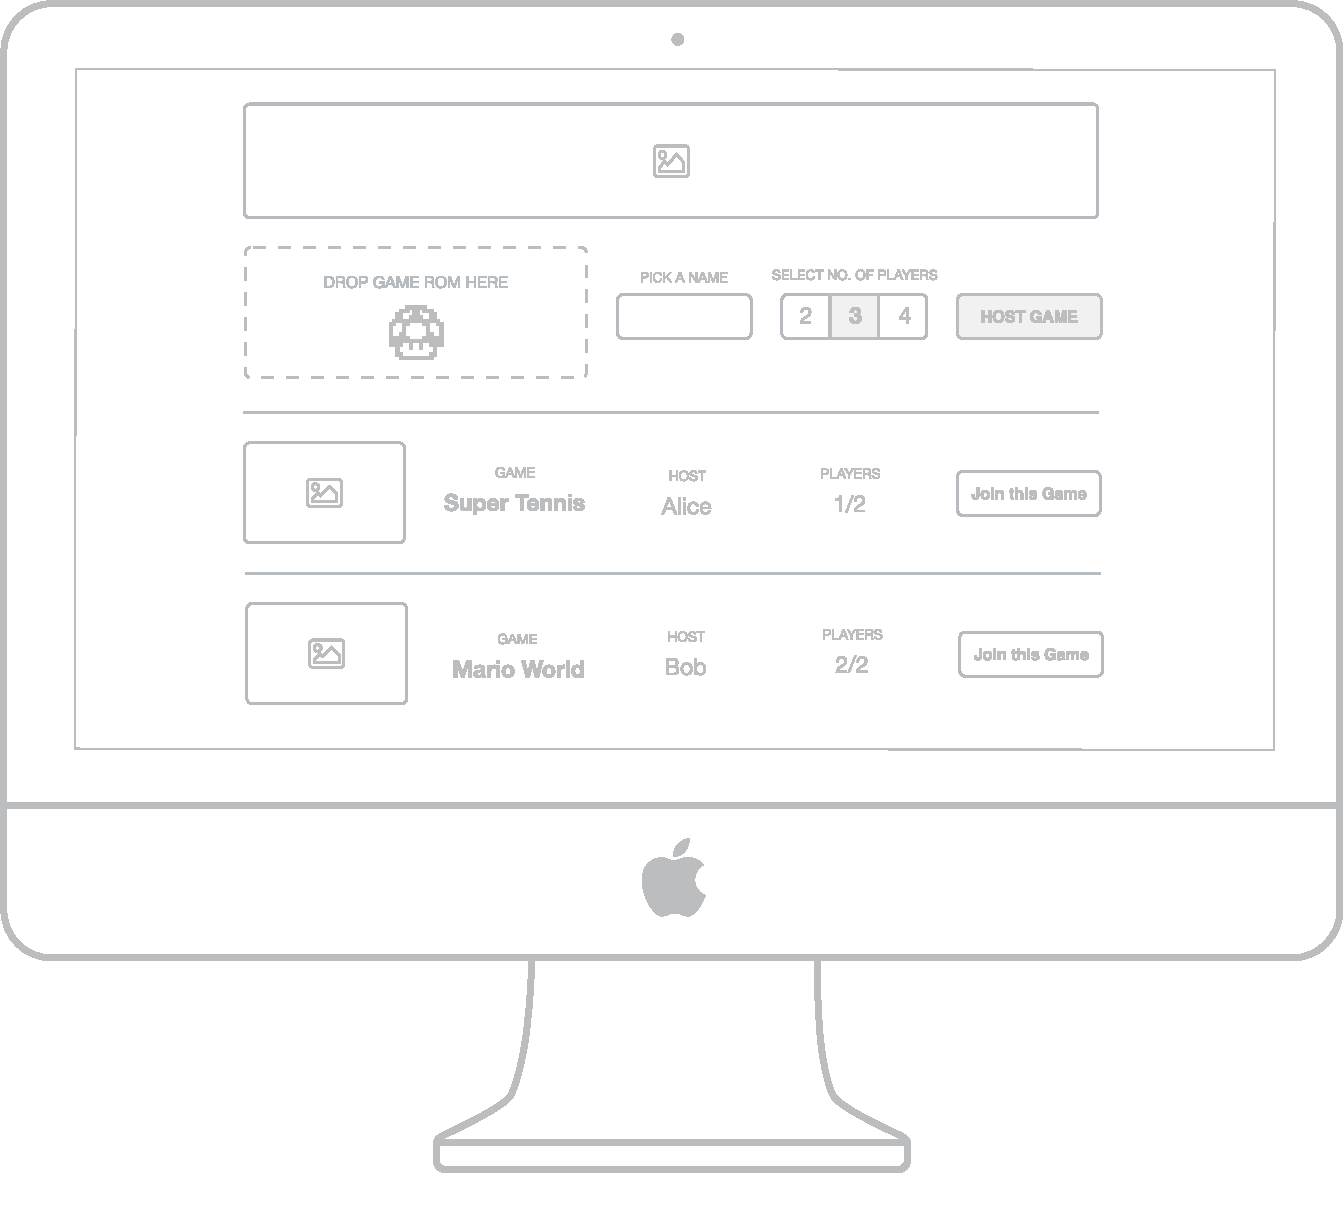
\includepdf[angle=270]{Abbildungen/Wireframes/1_Web_Match_List}
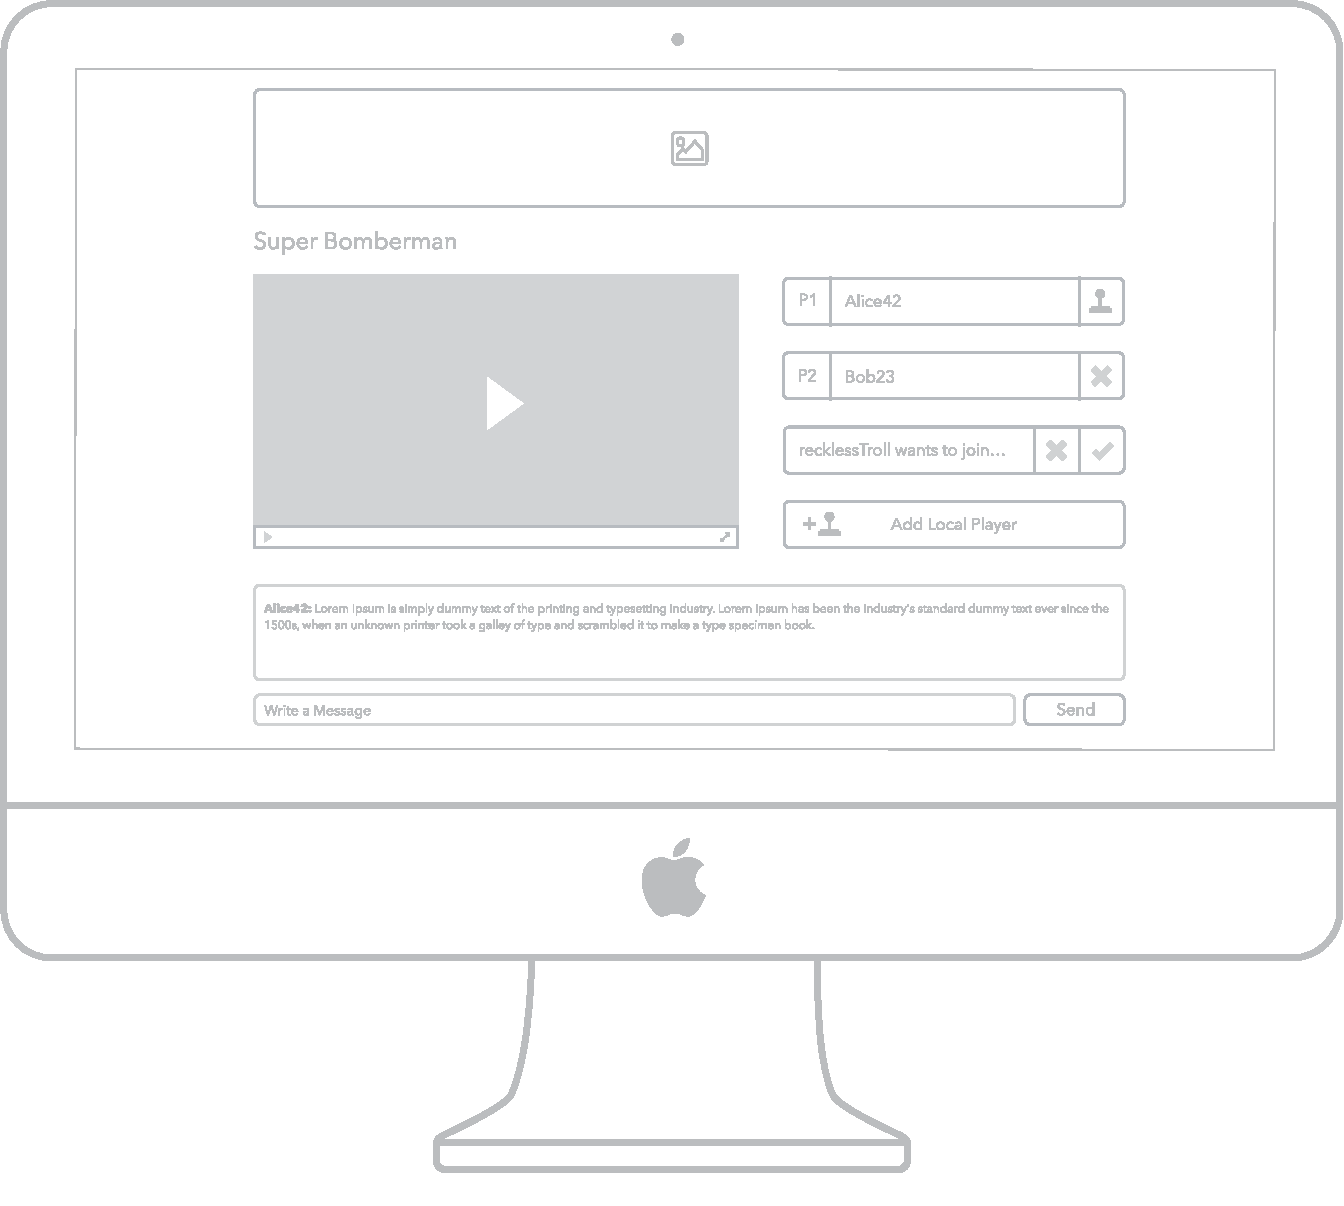
\includepdf[angle=90]{Abbildungen/Wireframes/2_Web_Match}
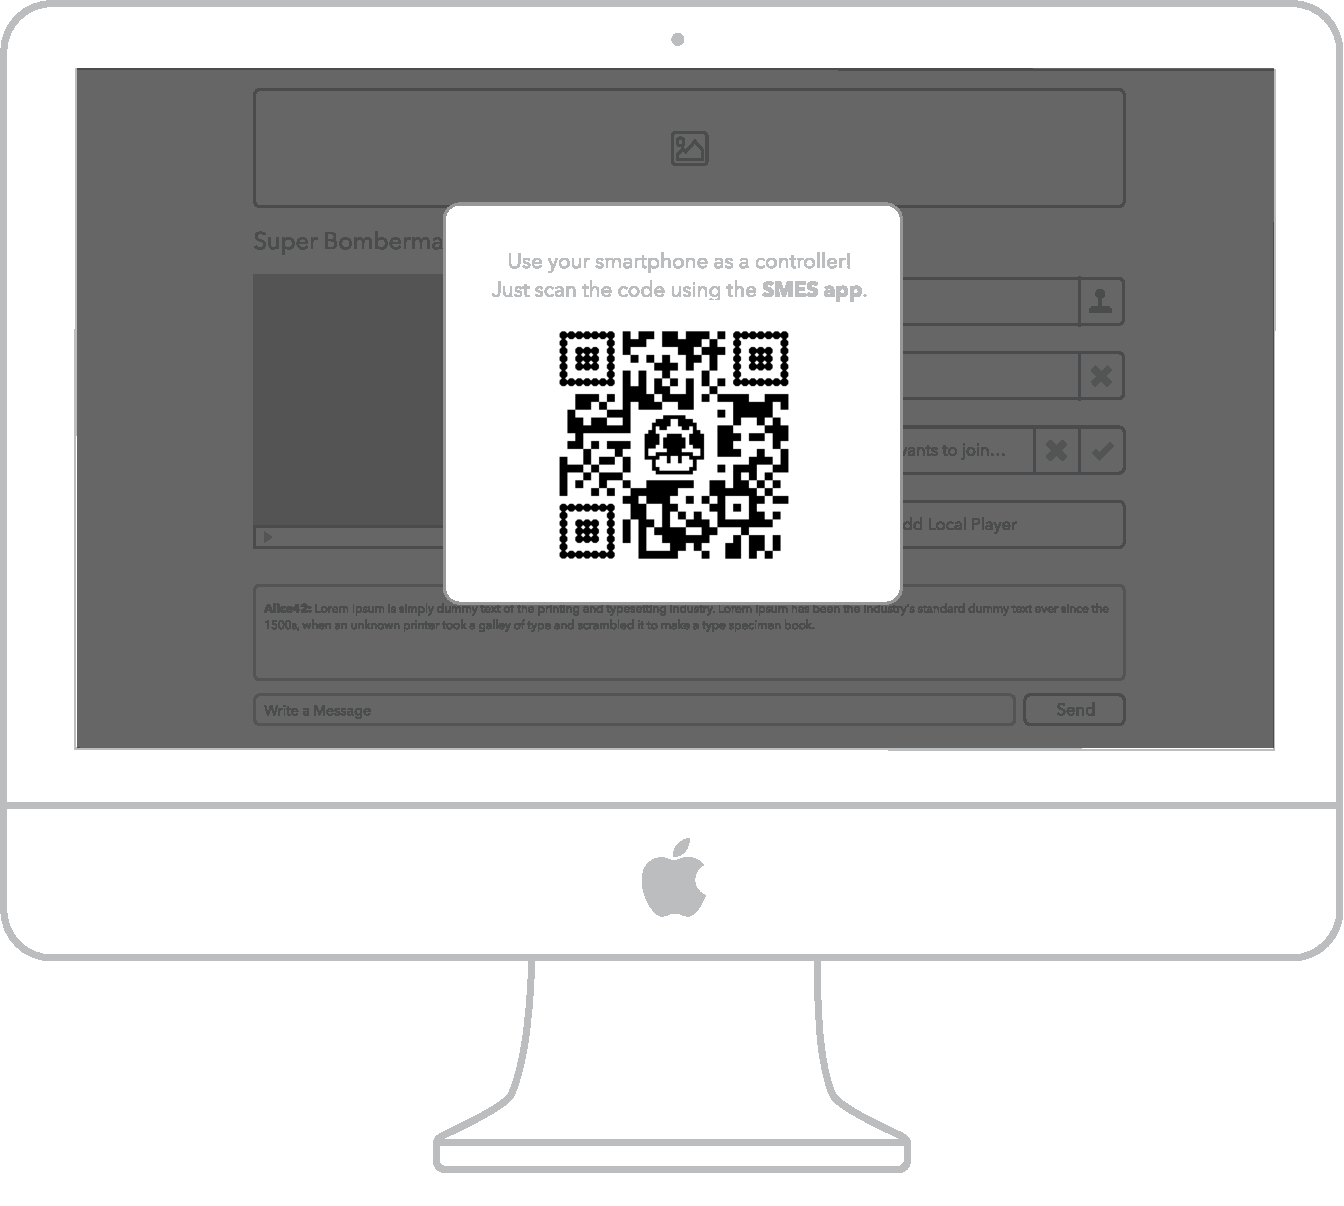
\includepdf[angle=270]{Abbildungen/Wireframes/3_Web_Match_Scan}
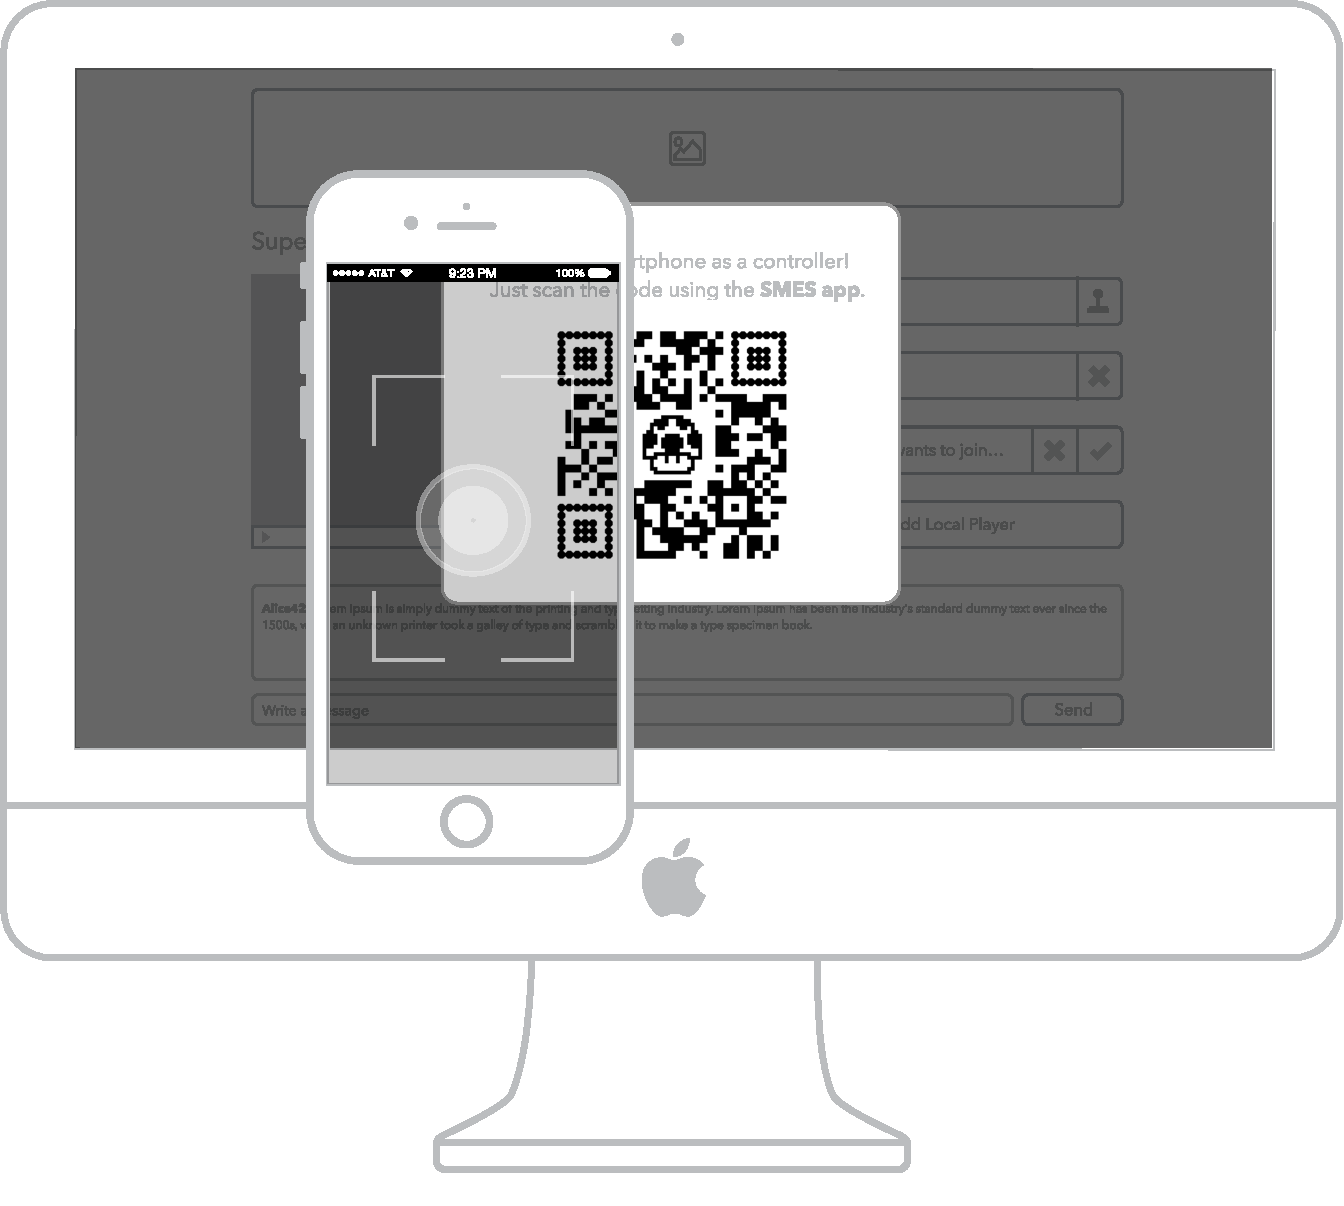
\includepdf[angle=90]{Abbildungen/Wireframes/4_Mobile_Scan}
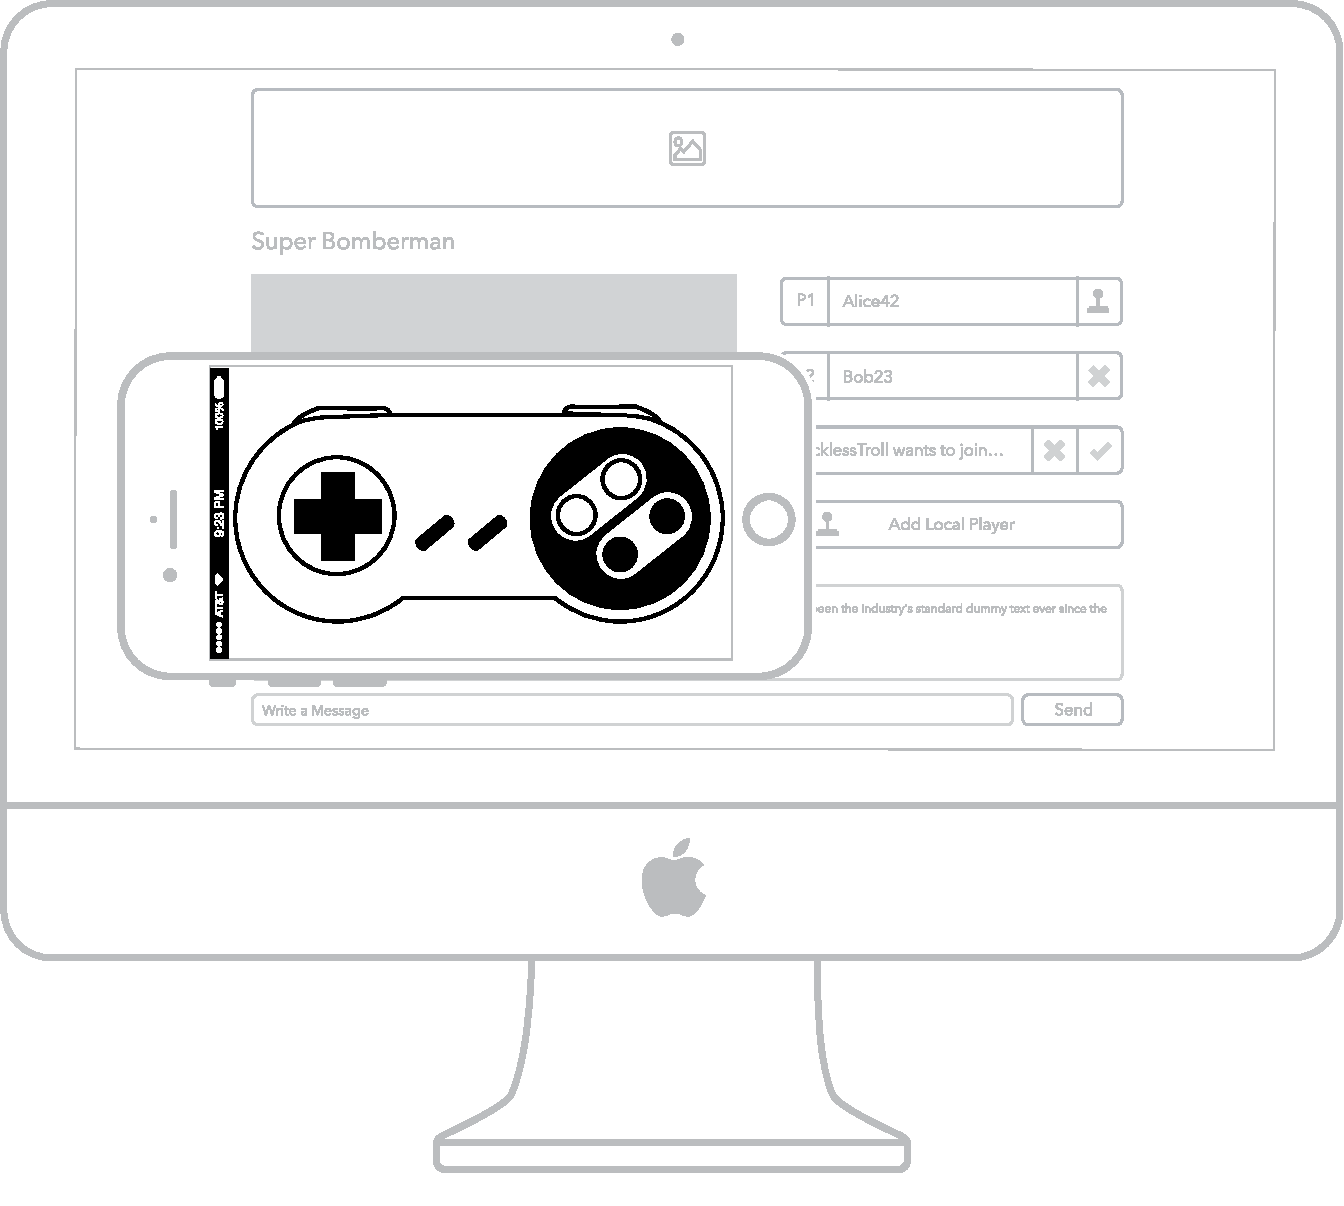
\includepdf[angle=270]{Abbildungen/Wireframes/5_Mobile_Play}

%\myfig{Abbildungen/Geraete/Macbook_Air_13}
%   {width=0.7\textwidth}
%   {This flower was photographed at my home town in 2010.}
%   {Home town flower}
%   {fig:flower}
%
%\myfig{Abbildungen/Geraete/Macbook_Pro_13}
%   {width=0.7\textwidth}
%   {This flower was photographed at my home town in 2010.}
%   {Home town flower}
%   {fig:flower}
%
%\myfig{Abbildungen/Geraete/iPhone_6}
%   {width=0.7\textwidth}
%   {This flower was photographed at my home town in 2010.}
%   {Home town flower}
%   {fig:flower}
%
%\myfig{Abbildungen/Geraete/HTC}
%   {width=0.7\textwidth}
%   {This flower was photographed at my home town in 2010.}
%   {Home town flower}
%   {fig:flower}

%%%

%\myfig{Abbildungen/Wireframes/1_Web_Match_List}
%   {width=0.9\textwidth}
%   {This flower was photographed at my home town in 2010.}
%   {Home town flower}
%   {fig:flower}
%
%\myfig{Abbildungen/Wireframes/2_Web_Match}
%   {width=0.9\textwidth}
%   {This flower was photographed at my home town in 2010.}
%   {Home town flower}
%   {fig:flower}
%
%\myfig{Abbildungen/Wireframes/3_Web_Match_Scan}
%   {width=0.9\textwidth}
%   {This flower was photographed at my home town in 2010.}
%   {Home town flower}
%   {fig:flower}
%
%\myfig{Abbildungen/Wireframes/4_Mobile_Scan}
%   {width=0.9\textwidth}
%   {This flower was photographed at my home town in 2010.}
%   {Home town flower}
%   {fig:flower}
%
%\myfig{Abbildungen/Wireframes/5_Mobile_Play}
%   {width=0.9\textwidth}
%   {This flower was photographed at my home town in 2010.}
%   {Home town flower}
%   {fig:flower}



\end{document}
